\documentclass[11pt,a4paper]{article}
\usepackage[T1]{fontenc}
\usepackage[utf8]{inputenc}
\usepackage{lmodern}
\usepackage[a4paper,margin=2.2cm]{geometry}
\usepackage{amsmath}
\usepackage{graphicx}
\usepackage{booktabs}
\usepackage{tabularx}
\usepackage{array}
\usepackage{float}
\usepackage{xcolor}
\usepackage[hidelinks]{hyperref}

\graphicspath{{figures/}}
\newcommand{\groupid}{XX}
\newcolumntype{R}{>{\raggedleft\arraybackslash}X}
\newcolumntype{L}{>{\raggedright\arraybackslash}X}
\setlength{\parskip}{4pt}
\setlength{\parindent}{0pt}
\renewcommand{\arraystretch}{1.12}

\title{\textbf{Who will subscribe? Ranking bank telemarketing calls}\\[4pt]
\large Machine Learning project 2026, DIA2, Group \groupid}
\author{Baudouin Parent \and Vivien Perrault \and Antonin Charron \and Enki Millet}
\date{November 2026}

\begin{document}
\maketitle

\begin{abstract}
A Portuguese bank sells term deposits by phone, and only 11.3\,\% of its calls end in a subscription. We built
models that score each client before the call so that the bank can call the most likely clients first. On the UCI
Bank Marketing data (41,176 calls after cleaning), a regularised logistic regression reaches a test PR-AUC of 0.454
[95\,\% CI 0.418, 0.488] and finds 64.0\,\% of the subscribers in the top 20\,\% of the list, above the 60\,\% goal we
set in week 1. A tuned random forest, LightGBM and a stacking ensemble raise the PR-AUC to 0.490--0.498 and the share
of subscribers reached to about 67\,\%; a paired bootstrap shows that this gain is real (+0.036 to +0.043, all
intervals above 0). A multilayer perceptron, our model outside the course, does not beat the baseline. When we train
on the oldest 80\,\% of the calls and test on the most recent 20\,\%, every flexible model falls below the logistic
regression (ROC-AUC 0.68 against 0.75), because the interest rate of the recent period lies outside the range seen
in training. Our recommendation therefore depends on how often the bank can retrain its model.
\end{abstract}

\tableofcontents
\newpage

%=====================================================================
\section{Business scope}

Telemarketing campaigns are expensive: each call takes an employee's time, and most clients refuse. The dataset
comes from a Portuguese bank that called clients between May 2008 and November 2010 to sell a term deposit
(Moro et al., 2014). If the bank knew in advance which clients are likely to subscribe, it could call them first and
spend the same call budget on far fewer refusals.

We chose this problem for our Data \& AI major because it covers the whole work of a data scientist on real data:
quality checks and statistical tests, a severe class imbalance, a leaking variable, a change of the data over time,
and a model whose output is turned into a business decision with a cost.

We fixed a measurable business goal in week 1, before training any model: \textbf{reach at least 60\,\% of the
subscribers by calling only 20\,\% of the clients}. Random calls would reach 20\,\%.

The project is split into four modules with one owner each (Table~\ref{tab:modules}).

\begin{table}[H]
\centering\small
\begin{tabularx}{\textwidth}{l L l}
\toprule
Module & Content & Owner \\
\midrule
1. Data exploration and cleaning & notebook 01, \texttt{bank\_clean.csv} & Baudouin Parent \\
2. Split, preprocessing, feature selection & \texttt{code/step2\_*.py}, notebook 05 & Vivien Perrault \\
3. Advanced models (v0.2--v0.4) & notebooks 03 and 06 & Antonin Charron \\
4. Baseline, AutoML v0.1, evaluation protocol & notebooks 02 and 04, \texttt{src/} & Enki Millet \\
\bottomrule
\end{tabularx}
\caption{Modules and owners (\texttt{ai\_governance/CONTRIBUTIONS.md}).}
\label{tab:modules}
\end{table}

%=====================================================================
\section{Problem formalisation and methods}

The research question is: \emph{before calling a client, can we predict whether they will subscribe, well enough
to rank the clients and call the best ones first?}

\begin{itemize}
\item Task: binary classification, used as a ranking. The model outputs a score per client (a probability of yes,
or a decision value for the linear SVM), and the bank calls the clients in decreasing order of score until its call
budget is spent.
\item Inputs: the 20 variables known before the call, minus \texttt{duration} (Section~\ref{sec:cleaning}): the
client (age, job, marital status, education, credit default, housing and personal loans), the contact (phone type,
month, day of the week, number of calls in this campaign), the previous campaign (days since the last contact,
number of contacts, outcome) and five economic indicators (employment variation rate, consumer price and confidence
indices, three-month Euribor rate, number of employees).
\item Target: $y=1$ if the client subscribed to the term deposit, 0 otherwise.
\item Evaluation: PR-AUC as main metric, recall in the top 20\,\% as business metric, 95\,\% bootstrap confidence
intervals and a paired bootstrap against the baseline (Section~\ref{sec:method}).
\end{itemize}

The method follows the four steps of the project: a baseline (logistic regression) and standard algorithms
(AutoML v0.1), then advanced versions: tree ensembles (v0.2), an ensemble of models (v0.3) and a model outside the
course (v0.4, a multilayer perceptron). Every model is chosen by cross-validation on the training set and evaluated
once on the test set, then on a temporal split.

%=====================================================================
\section{Data description and exploration}

\subsection{Source and content}
We use \texttt{bank-additional-full.csv} from the UCI Machine Learning Repository (CC BY 4.0 licence): 41,188 calls,
20 input variables (10 categorical, 10 numerical) and the target $y$. The data exploration and cleaning are in
notebook 01 (module 1).

\subsection{Missing values}
There are no empty cells, but missing values are coded as the string \texttt{unknown}: 20.9\,\% of \texttt{default}, 4.2\,\% of
\texttt{education}, 2.4\,\% of \texttt{housing} and \texttt{loan}, 0.8\,\% of \texttt{job}. They are not missing at
random. For \texttt{default}, the clients with \texttt{unknown} subscribe at 5.2\,\% against 12.9\,\% for the others
($\chi^2$, $p<0.001$), so \texttt{unknown} carries information and we keep it as a category instead of imputing it.
\texttt{pdays} $=999$ is a second hidden missing value: it means ``never contacted before'' for 96.3\,\% of the rows
(see below).

\subsection{Imbalanced data}\label{sec:imbalance}
4,640 calls are a yes (11.3\,\%). A model that always answers no has an accuracy of 88.7\,\%, so accuracy cannot
measure anything here. We handle the imbalance in four places, without resampling: stratified splits and folds (the
share of yes is the same in every part), a ranking metric that focuses on the yes (PR-AUC), no reweighting of the
logistic regression (Section~\ref{sec:baseline}) and a decision threshold chosen on out-of-fold scores
(Section~\ref{sec:threshold}).

\subsection{Outliers and skewed variables}
By the interquartile-range rule, \texttt{campaign} has 2,406 outliers, \texttt{previous} 5,625 and \texttt{age} 468.
They look real (a client called 56 times, a client aged 98) and not like input errors, so we keep them. Tree
models are not sensitive to them; for the linear models we reduce the skew of \texttt{campaign} (skewness 4.8) with
$\log(1+x)$, which brings it to 1.35 and the number of outliers to 869.

\subsection{Leakage and cleaning}\label{sec:cleaning}
The cleaning steps are all row by row, so they can be applied before the train/test split without leaking
information from the test rows:
\begin{itemize}
\item \texttt{duration} (length of the call) is removed. It is known only after the call, when the answer is already
known (a call of 0 seconds is always a no), and the dataset documentation itself warns against using it
(Figure~\ref{fig:duration}).
\item \texttt{pdays} $=999$ means ``never contacted before'' for 96.3\,\% of the rows. Used as a number, 999 would
look like a very long delay, so we split it into a binary \texttt{prev\_contacted} and the number of days
(\texttt{pdays\_clean}, $-1$ when never contacted).
\item \texttt{campaign} is replaced by $\log(1+\texttt{campaign})$.
\item 12 exact duplicate rows are removed, which leaves 41,176 calls.
\end{itemize}

\begin{figure}[H]
\centering
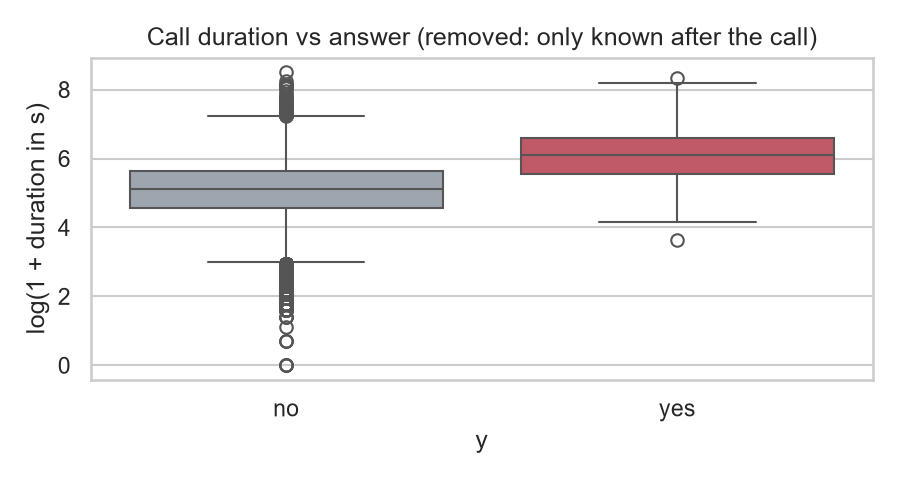
\includegraphics[width=0.62\textwidth]{duration_leak.png}
\caption{Length of the call by answer. Calls that end in a yes are much longer: \texttt{duration} would let a
model ``see'' the answer, so it is excluded.}
\label{fig:duration}
\end{figure}

\subsection{Statistical analysis of the variables}
With 41,000 rows almost every test is significant, so we compare variables by the strength of their link with the
target, not by their p-value.

\textbf{Categorical variables.} The $\chi^2$ test of independence assumes an expected count of at least 5 in every
cell. This condition failed for \texttt{default} (3 rows with \texttt{yes}, minimum expected count 0.34) and
\texttt{education} (18 rows with \texttt{illiterate}). Grouping the rare categories into \texttt{other} was not
enough, because each variable has a single rare category; these 3 and 18 rows are left out of the test, and an
\texttt{assert} now checks the condition. The strongest links (Cramér's V) are the outcome of the previous campaign
(\texttt{poutcome}, 0.32), the month (0.27), the job (0.15) and the type of phone (0.14). \texttt{housing}
($p=0.057$) and \texttt{loan} ($p=0.58$) are not linked to the target.

\textbf{Numerical variables.} The D'Agostino--Pearson test rejects normality for every numerical variable
($p\approx0$), so we use the Mann--Whitney test instead of a t-test, with the rank-biserial correlation $r$ as effect
size. The three economic indicators have by far the strongest links: \texttt{nr.employed} ($r=-0.50$),
\texttt{euribor3m} ($-0.49$) and \texttt{emp.var.rate} ($-0.43$). Client variables are weak in comparison
(\texttt{campaign}: $-0.11$, age: $-0.02$).

\textbf{Collinearity.} \texttt{euribor3m}, \texttt{emp.var.rate} and \texttt{nr.employed} are correlated above 0.9
(variance inflation factors 64.5, 33.3 and 31.7). We keep all three: tree models are not affected, and the logistic
regression is regularised. We do not interpret their coefficients one by one.

\subsection{Drift over time}
The rows are in chronological order. The share of yes rises from 2.8\,\% in the first tenth of the file to 45.9\,\% in
the last (Figure~\ref{fig:drift}): after the 2008 crisis the bank made fewer but better-targeted calls, and the
economic indicators moved at the same time. This has two consequences for the whole project. First, the row order
is the time order and must never become a feature (an \texttt{assert} in \texttt{src/common.py} checks that
\texttt{row\_order} and \texttt{duration} are not features). Second, a random split mixes old and recent calls, so
we also test every model on a temporal split (Section~\ref{sec:drift}).

\begin{figure}[H]
\centering
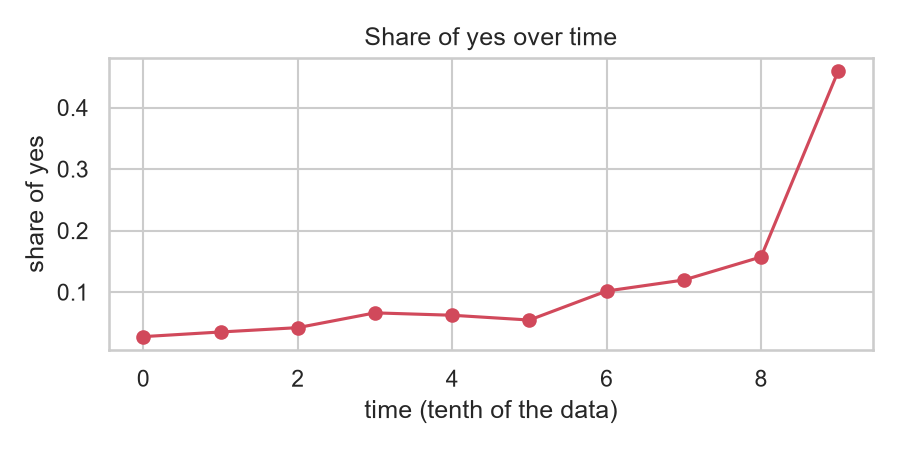
\includegraphics[width=0.6\textwidth]{temporal_drift.png}
\caption{Share of yes in each tenth of the file (chronological order).}
\label{fig:drift}
\end{figure}

%=====================================================================
\section{Methodology}\label{sec:method}

\subsection{Data splitting for train and test}
The data is split once (\texttt{code/step2\_split.py}) into a training set of 32,940 calls and a test set of 8,236
calls (928 yes), stratified on $y$ with seed 42. An \texttt{assert} checks that no row is in both sets. All choices
(model, hyperparameters, decision threshold) are made by 5-fold stratified cross-validation on the training set; the
folds are shuffled, otherwise each fold would be a period of time. The test set is scored once, in notebook 04, after
every choice has been made. As a second test, every model is also trained on the oldest 80\,\% of the calls and
tested on the most recent 20\,\%.

\subsection{Preprocessing without leakage (module 2)}
Every model is a scikit-learn \texttt{Pipeline}: a \texttt{ColumnTransformer} (one-hot encoding of the 10
categorical variables with categories of fewer than 20 rows grouped together, standardisation of the numerical
variables, binary variables passed through), followed by the model. The whole pipeline is given to every
cross-validation function, so the encoder and the scaler are refitted on the four training folds of each split and
the validation fold never contributes to them. After encoding, the model sees 63 columns.

\subsection{Metrics}
\begin{itemize}
\item PR-AUC (average precision) is the main metric. It measures whether the yes are at the top of the
ranking and does not reward the many easy no. A random ranking scores the share of yes (0.113).
\item Recall in the top 20\,\% is the business metric: the share of all subscribers reached when the bank
calls the 20\,\% best-scored clients. Clients tied at the cut are counted as random picks (Section~\ref{sec:ties}).
\item ROC-AUC is reported for comparison with the literature and for the temporal split, because unlike
PR-AUC it does not depend on the share of yes.
\item Precision, recall and F1 are computed at a decision threshold. The threshold maximises F1 on out-of-fold scores of
the training set (\texttt{cross\_val\_predict}); it is never chosen on the test set.
\end{itemize}

\subsection{Uncertainty}
A test score comes from one sample of 8,236 clients. We give a 95\,\% confidence interval from 1,000 bootstrap
resamples of the test rows (with replacement, percentile method). To compare a model with the baseline we use a
paired bootstrap: both models are scored on the same resampled rows and we take the 2.5 and 97.5 percentiles of the
difference. Pairing matters here: the intervals of the random forest [0.461, 0.530] and of the baseline [0.418,
0.488] overlap, yet the paired difference is clearly positive, because a ``hard'' resample lowers both scores at the
same time. These intervals only cover the sampling of the test set, not the randomness of training.

%=====================================================================
\section{Algorithm description}

\begin{itemize}
\item \emph{Logistic regression} models the log-odds of a yes as a linear function of the inputs,
$\log\frac{P(y=1)}{P(y=0)} = w_0 + w^\top x$, and fits $w$ by minimising the log-loss plus an L2 penalty on $w$ whose
strength is $1/C$.
\item \emph{Linear SVM} looks for the hyperplane that separates the classes with the largest margin (hinge loss,
L2 penalty). It outputs a signed distance to the hyperplane, not a probability, which is enough to rank clients.
\item \emph{Decision tree} splits the data recursively on the variable and threshold that most reduce the impurity
(Gini or entropy); a leaf predicts the share of yes among its training rows.
\item \emph{k-nearest neighbours} scores a client by the share of yes among its $k$ closest training clients
(Euclidean distance on the standardised features).
\item \emph{Gaussian Naive Bayes} applies Bayes' rule assuming the inputs are independent given the class, each
with a Gaussian distribution.
\item \emph{Random forest} (bagging) averages many deep trees, each trained on a bootstrap sample of the rows and
choosing each split among a random subset of the variables. Averaging decorrelated trees lowers the variance of a
single tree.
\item \emph{LightGBM} (gradient boosting) builds small trees one after the other; each new tree is fitted to the
gradient of the log-loss of the current ensemble, and its contribution is shrunk by a learning rate. Trees grow
leaf by leaf on histograms of the variables, which makes training fast.
\item \emph{Stacking} (Wolpert, 1992) trains a meta-model on the predictions of several base models; the meta-model
must learn on predictions made for rows the base models did not see.
\item \emph{Multilayer perceptron} stacks layers of neurons; each computes a weighted sum of its inputs followed by
the ReLU function $\max(0,z)$, and the output neuron applies a sigmoid. The weights are learned by back-propagation
with the Adam optimiser on the log-loss, with an L2 penalty $\alpha$. With no hidden layer it is a logistic
regression.
\end{itemize}

%=====================================================================
\section{Algorithm implementation and hyperparameters}

\subsection{Dummy model}
A model that gives every client the same score (the share of yes) has a PR-AUC of 0.113, a ROC-AUC of 0.5 and reaches
20\,\% of the subscribers with 20\,\% of the calls. It is the floor, and it also served as a test of our own metric
code (Section~\ref{sec:ties}).

\subsection{Baseline: logistic regression}\label{sec:baseline}
The baseline is a logistic regression with an L2 penalty. We tuned the inverse regularisation strength $C$ over
$\{0.001, \dots, 100\}$ and \texttt{class\_weight} over \{None, balanced\} with a grid search on the 5 folds.

\textbf{Choice of $C$.} The CV PR-AUC is flat for $C\geq0.1$ (0.4484 at $C=0.1$, 0.4497 at $C=100$), and the best value
of the grid was its last one, $C=100$; a first grid stopping at 10 had picked 10. A difference of 0.001 is smaller
than the standard deviation between folds (about 0.006), so taking the maximum would be choosing on noise, and
choosing the weakest regularisation for collinear variables. We use the one-standard-error rule: among the settings
whose score is within one standard error of the best, we keep the most regularised one. The standard error is the
sample standard deviation of the 5 fold scores divided by $\sqrt5$; scikit-learn reports the population standard
deviation, so we multiply it by $\sqrt{5/4}$. The threshold is $0.4497-0.0030=0.4468$, which selects $C=0.1$.

\textbf{Class weights.} Balanced weights rank the clients almost the same way (out-of-fold PR-AUC 0.445 against
0.448) but distort the probabilities: the mean predicted probability becomes 0.392 for a real share of 0.113, and the
Brier score doubles (0.079 to 0.165, Figure~\ref{fig:calib}). We keep \texttt{class\_weight=None}; the imbalance is
handled by the metric and by the threshold.

\begin{figure}[H]
\centering
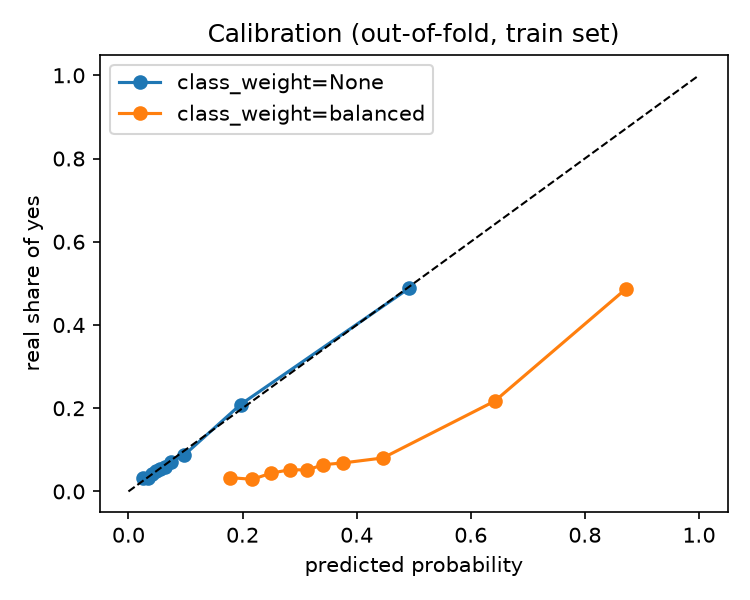
\includegraphics[width=0.42\textwidth]{logreg_calibration.png}\hspace{0.03\textwidth}
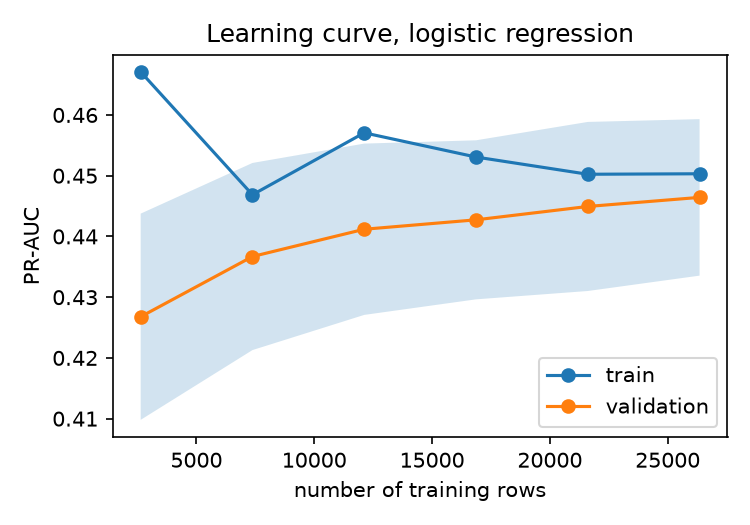
\includegraphics[width=0.5\textwidth]{logreg_learning_curve.png}
\caption{Left: calibration of the out-of-fold probabilities with and without balanced class weights. Right:
learning curve of the baseline.}
\label{fig:calib}
\end{figure}

\textbf{Fit.} Train and CV PR-AUC are close (0.456 against 0.448) and the learning curve is flat after about 20,000
rows: the model does not overfit, it is limited by its linear frontier. More data would not help much; a more
flexible model might. The signs of the coefficients make sense: calls in March and December work better, calls in May
(the busiest month) and to landlines work worse, a client contacted in a previous campaign is more likely to say yes
unless that campaign failed, and a high employment variation rate pushes the probability down.

\textbf{Benchmark.} Moro et al.\ (2014) report an AUC of about 0.8 on this problem with a neural network. Their
setting differs (more years, 22 features selected among 150, test on the most recent contacts), so we use it as an
order of magnitude. Our baseline has a cross-validated ROC-AUC of 0.789 and a PR-AUC of 0.448, and it reaches
61.8\,\% of the subscribers in the top 20\,\% out-of-fold, above the 60\,\% goal.

\subsection{AutoML v0.1: standard algorithms}
We ran a random search, with the same pipeline, folds and score, over the algorithms seen in class
(Table~\ref{tab:v01}). None beats the baseline. Naive Bayes is clearly below because it assumes independent
variables, which is false for the three economic indicators. The decision tree is the only model that starts to
overfit (gap 0.023) even with at least 166 rows per leaf. The KNN needs 275 neighbours and ten times more search time
for no gain. All models stay at PR-AUC 0.43--0.45: simple models hit a ceiling.

\begin{table}[H]
\centering\small
\begin{tabularx}{0.8\textwidth}{L r r r}
\toprule
Model & CV PR-AUC (mean $\pm$ std) & CV ROC-AUC & Train $-$ CV \\
\midrule
Dummy & 0.113 & 0.500 & \\
\textbf{Logistic regression (baseline, $C=0.1$)} & \textbf{0.448 $\pm$ 0.006} & 0.789 & 0.007 \\
Linear SVM & 0.446 $\pm$ 0.008 & 0.785 & 0.006 \\
Decision tree & 0.439 $\pm$ 0.008 & 0.783 & 0.023 \\
k-nearest neighbours & 0.432 $\pm$ 0.011 & 0.784 & 0.008 \\
Gaussian Naive Bayes & 0.390 $\pm$ 0.013 & 0.772 & 0.001 \\
\bottomrule
\end{tabularx}
\caption{AutoML v0.1, 5-fold cross-validation on the training set (\texttt{results/cv\_step2.csv}).}
\label{tab:v01}
\end{table}

\subsection{v0.2: random forest and LightGBM}
Tree ensembles can learn interactions (month $\times$ economy, previous contact $\times$ economy) that a linear model
cannot. With its default settings the random forest grows every tree until its leaves are pure and learns the
training folds by heart: train PR-AUC 0.999 against 0.403 in CV, below the baseline. A validation curve on the maximum
depth (Figure~\ref{fig:depth}) shows underfitting at depth 2 to 4, the best validation score at depth 8 to 10 (0.460,
0.461) and overfitting from depth 14, where the train score keeps rising (0.76, then 0.96 at depth 20) while the
validation score falls.

\begin{figure}[H]
\centering
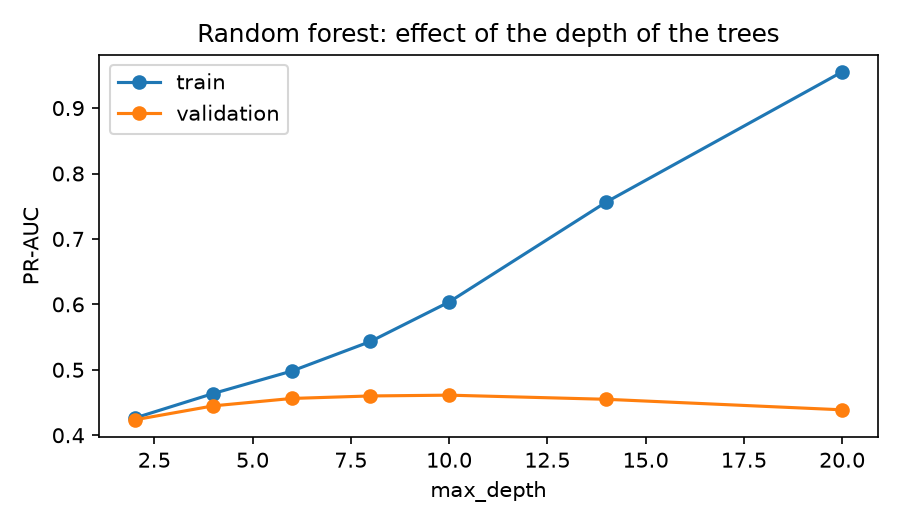
\includegraphics[width=0.55\textwidth]{rf_max_depth.png}
\caption{Random forest: train and validation PR-AUC against the maximum depth (5 folds).}
\label{fig:depth}
\end{figure}

We tuned both models with \texttt{RandomizedSearchCV} (10 combinations each, same folds, PR-AUC). The random forest
keeps depth 10, at least 11 rows per leaf, half of the features per split and balanced class weights (CV 0.465, gap
0.11). LightGBM keeps 205 trees of 11 leaves, a learning rate of 0.025 and at least 73 rows per leaf (CV 0.467, gap
0.04, against 0.457 and 0.17 with its defaults). LightGBM reaches the same score with a much smaller gap and fits
eight times faster.

\subsection{Feature selection}
Notebook 05 compares all the features with two mutual-information filters (best 50\,\% or 75\,\% of the encoded
columns) and two L1-based selections (an L1-penalised logistic regression keeps the columns whose coefficient is
above the median, or above 1.25 times the mean). The selector is a pipeline step, refitted inside each fold. The best
method, L1 with the median threshold, keeps 32 of the 63 columns and gains 0.0004 in CV; on the test set the paired
difference is +0.0012 [$-0.0004$, +0.0029]. The interval contains 0, so we keep all the features. The L1 selector
also illustrates the collinearity: it drops \texttt{nr.employed} and keeps \texttt{emp.var.rate}, an arbitrary
choice between two near copies.

\subsection{v0.3: ensembles}
Soft voting averages the probabilities of the logistic regression, the random forest and LightGBM. Stacking
(Wolpert, 1992) trains a second logistic regression on their scores. The meta-model must learn on out-of-fold
scores (\texttt{StackingClassifier(cv=cv\_folds())}): on its own training rows the random forest scores 0.57 against
0.47 in CV, and a meta-model fitted on those scores would trust it too much. Stacking reaches 0.470 in CV and soft
voting 0.468, so stacking is the ensemble sent to the test set. Its gain over LightGBM alone (+0.003) is below the
standard deviation between folds, for about 50 times the fitting time. The meta-model weights (random forest 3.48,
LightGBM 1.64, logistic regression 0.70) show why: two of the three members are tree ensembles trained on the same
variables, so they make similar errors.

\subsection{v0.4: a model outside the course, the multilayer perceptron}
Moro et al.\ (2014) found a neural network to be the best model on this dataset, and Kadra et al.\ (2021) showed that
simple MLPs compete on tabular data when their regularisation is tuned. We used scikit-learn's
\texttt{MLPClassifier} (ReLU hidden layers, sigmoid output, Adam, L2 penalty $\alpha$). By default it overfits
(train 0.74, CV 0.37). Its \texttt{early\_stopping} option keeps the epoch with the best validation accuracy, which
barely moves when 88.7\,\% of the answers are no, so we switched it off and tuned the number of epochs together with
$\alpha$, the layer sizes, the learning rate and the batch size (20 combinations). The best network has layers of 128
and 64 units, $\alpha=0.01$ and 80 epochs: CV PR-AUC 0.453, level with the baseline. This agrees with Grinsztajn et
al.\ (2022), who found tree-based models ahead of neural networks on typical tabular data.

\begin{figure}[H]
\centering
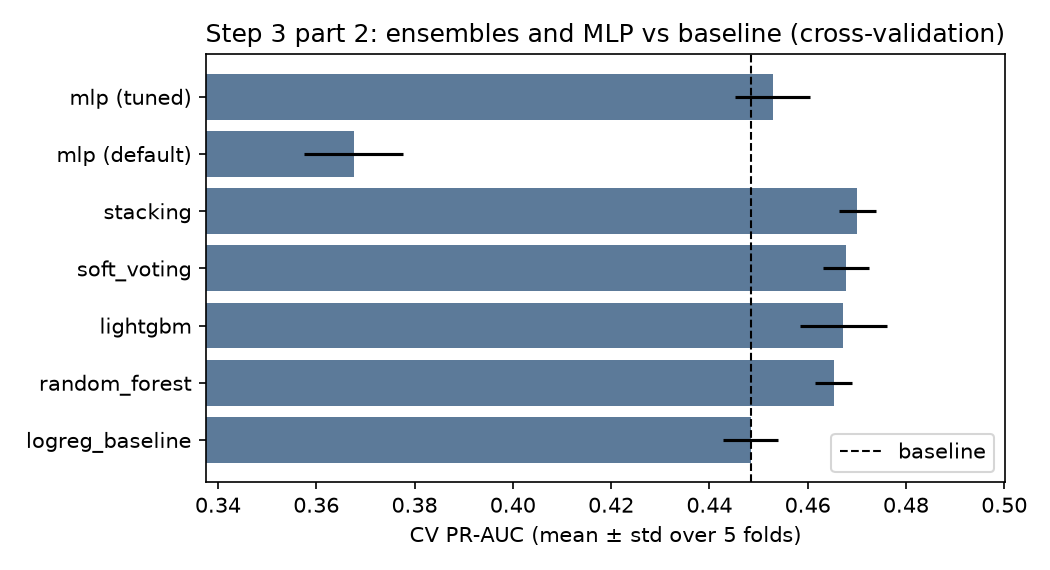
\includegraphics[width=0.66\textwidth]{cv_step3_part2.png}
\caption{Cross-validated PR-AUC (mean $\pm$ std over 5 folds) of the baseline, the v0.2 models, the ensembles and
the MLP. The dashed line is the baseline.}
\label{fig:cvstep3}
\end{figure}

%=====================================================================
\section{Results}

Every model of Table~\ref{tab:test} was chosen by cross-validation, refitted on the whole training set and scored
once on the test set. The soft voting ensemble lost to stacking in CV and was never tested.

\begin{table}[H]
\centering\small
\begin{tabularx}{\textwidth}{L c c c c}
\toprule
Model & CV PR-AUC & Test PR-AUC [95\,\% CI] & ROC-AUC & Reached at 20\,\% [95\,\% CI] \\
\midrule
Dummy & 0.113 & 0.113 [0.105, 0.120] & 0.500 & 20.0\,\% \\
Logistic regression (baseline) & 0.448 & 0.454 [0.418, 0.488] & 0.800 & 64.0\,\% [61.2, 66.9] \\
Linear SVM & 0.446 & 0.449 [0.412, 0.484] & 0.797 & 64.3\,\% [61.1, 67.0] \\
k-nearest neighbours & 0.432 & 0.448 [0.413, 0.481] & 0.800 & 65.2\,\% [62.0, 68.1] \\
Decision tree & 0.439 & 0.472 [0.434, 0.503] & 0.805 & 64.0\,\% [60.9, 66.8] \\
Naive Bayes & 0.390 & 0.399 [0.365, 0.432] & 0.782 & 61.2\,\% [58.1, 63.8] \\
\midrule
Random forest (v0.2) & 0.465 & \textbf{0.498} [0.461, 0.530] & 0.817 & \textbf{67.1}\,\% [64.1, 69.8] \\
LightGBM (v0.2) & 0.467 & 0.490 [0.453, 0.523] & 0.814 & 66.6\,\% [63.7, 69.3] \\
Stacking (v0.3) & \textbf{0.470} & 0.495 [0.458, 0.527] & 0.817 & 66.9\,\% [63.7, 69.5] \\
MLP (v0.4) & 0.453 & 0.467 [0.432, 0.502] & 0.804 & 65.2\,\% [62.1, 67.8] \\
\bottomrule
\end{tabularx}
\caption{Test set, 8,236 calls (\texttt{results/test\_comparison.csv}).}
\label{tab:test}
\end{table}

\subsection{Overfitting, underfitting and imbalance}
Table~\ref{tab:gaps} gathers the train and cross-validation scores of the main models. The logistic regression
underfits slightly (train and CV close, flat learning curve). The default random forest, the default LightGBM and the
default MLP overfit strongly; regularising them (depth and leaf size for the trees, number of leaves for LightGBM,
$\alpha$ and the number of epochs for the MLP) closes most of the gap and raises the CV score. Among the tuned models
LightGBM has the smallest gap. The imbalance is handled as described in Section~\ref{sec:imbalance}: no model is
evaluated with accuracy, and every threshold is chosen out-of-fold.

\begin{table}[H]
\centering\small
\begin{tabular}{l c c c l}
\toprule
Model & Train PR-AUC & CV PR-AUC & Gap & Diagnosis \\
\midrule
Logistic regression & 0.456 & 0.448 & 0.007 & slight underfitting \\
Decision tree (tuned) & 0.462 & 0.439 & 0.023 & starts to overfit \\
Random forest, default & 0.999 & 0.403 & 0.596 & strong overfitting \\
Random forest, tuned & 0.572 & 0.465 & 0.106 & moderate \\
LightGBM, default & 0.631 & 0.457 & 0.174 & overfitting \\
LightGBM, tuned & 0.504 & 0.467 & 0.036 & good \\
Stacking & 0.544 & 0.470 & 0.074 & moderate \\
MLP, default & 0.741 & 0.368 & 0.373 & strong overfitting \\
MLP, tuned & 0.534 & 0.453 & 0.082 & moderate \\
\bottomrule
\end{tabular}
\caption{Train and cross-validated PR-AUC (5 folds, \texttt{results/cv\_step2.csv}, \texttt{cv\_step3.csv},
\texttt{cv\_step3\_part2.csv}).}
\label{tab:gaps}
\end{table}

\subsection{Evaluation and comparison with the baseline}
Table~\ref{tab:paired} gives the paired bootstrap differences with the baseline. The random forest, LightGBM and the
stacking beat it on both metrics, with intervals above 0. Their one-sided bootstrap p-value is below 0.001 for both
metrics, so they stay significant even after a Bonferroni correction for the 16 comparisons of the table. The three
cannot be separated from each other: random forest minus LightGBM is +0.007 [$-0.003$, +0.017], and their order
changes between CV and test. The MLP does not show a reliable gain: its PR-AUC difference is +0.013 [$-0.001$,
+0.026]; its one-sided p-value is 0.038, but the two-sided interval contains 0 and we keep the criterion fixed
beforehand.

On the test set the PR-AUC of the decision tree is above the baseline (+0.017 [0.001, 0.034]), but the tree was
below the baseline in CV, it does not reach more subscribers ($-0.2$ points), and with 16 comparisons one of them is
expected to pass by chance. We base model choices on cross-validation and use the test set only to confirm them.

\begin{table}[H]
\centering\small
\begin{tabular}{l c c}
\toprule
Model minus baseline & $\Delta$ PR-AUC [95\,\% CI] & $\Delta$ reached with 20\,\% of calls [95\,\% CI] \\
\midrule
Random forest & +0.043 [0.029, 0.057] & +2.8 points [1.2, 4.4] \\
Stacking & +0.040 [0.029, 0.050] & +2.6 points [1.1, 4.1] \\
LightGBM & +0.036 [0.024, 0.047] & +2.5 points [1.2, 3.8] \\
MLP & +0.013 [$-0.001$, 0.026] & +1.0 point [$-0.4$, 2.5] \\
Decision tree & +0.017 [0.001, 0.034] & $-0.2$ points [$-1.9$, 1.3] \\
k-nearest neighbours & $-0.007$ [$-0.022$, 0.008] & +0.9 points [$-0.5$, 2.3] \\
Linear SVM & $-0.005$ [$-0.011$, 0.001] & +0.2 points [$-0.6$, 0.9] \\
Naive Bayes & $-0.056$ [$-0.073$, $-0.038$] & $-3.0$ points [$-5.1$, $-1.1$] \\
\bottomrule
\end{tabular}
\caption{Paired bootstrap against the baseline on the test set (1,000 resamples, \texttt{results/paired\_vs\_baseline.csv}).}
\label{tab:paired}
\end{table}

\subsection{What it means for the bank}
On the test set, calling the top 20\,\% means 1,648 calls. Random calls would reach about 186 of the 928 subscribers.
The baseline reaches 594 (precision 36\,\%), the random forest 623 (precision 38\,\%), so the step 3 models find about
29 more subscribers for the same number of calls. Figure~\ref{fig:gain} shows that every model is above the 60\,\%
line at 20\,\% of calls; the curves of the best models are close to each other over the whole range.

\begin{figure}[H]
\centering
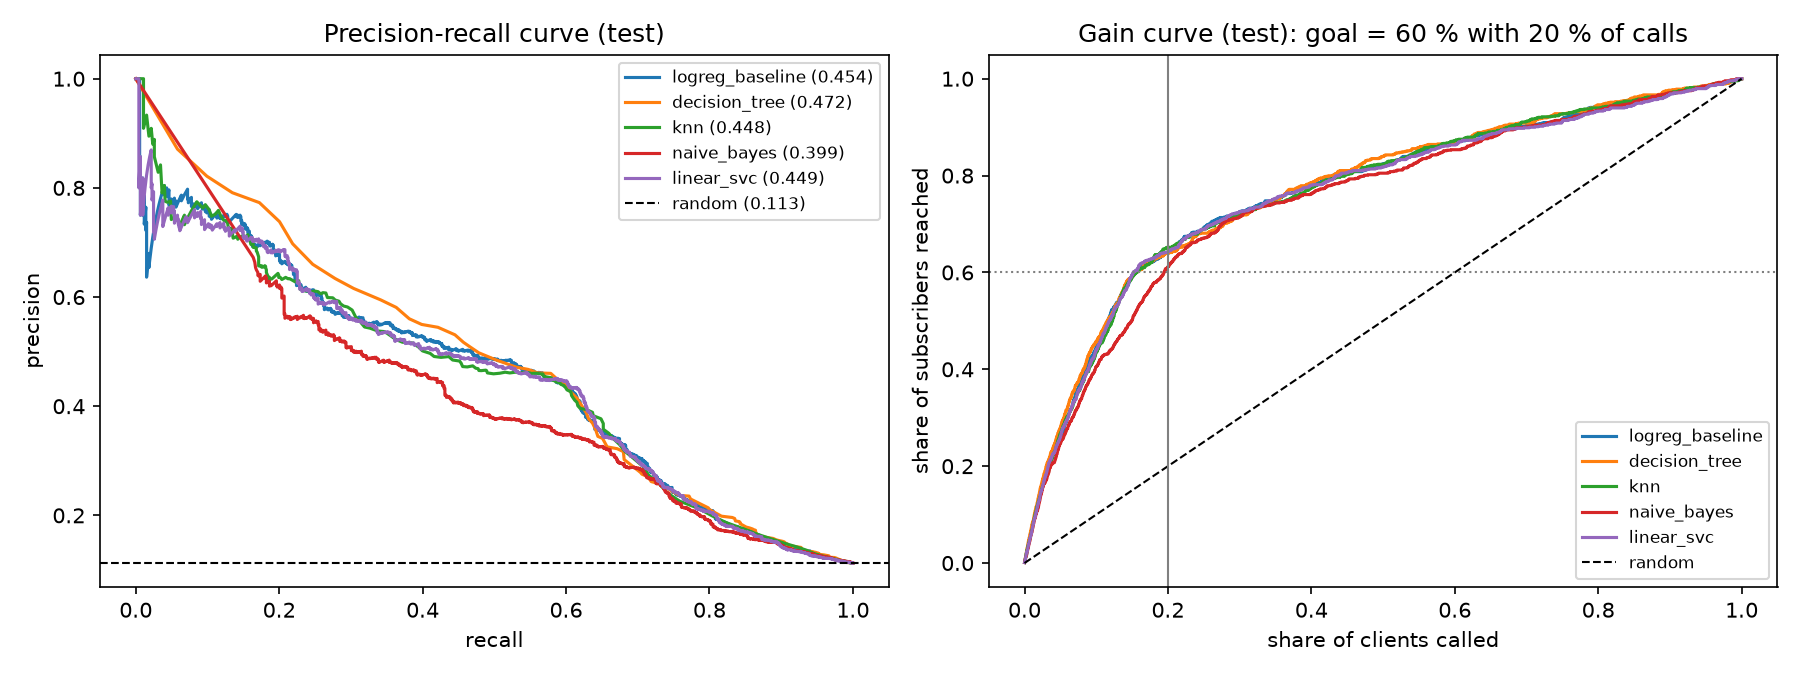
\includegraphics[width=\textwidth]{test_pr_gain_curves.png}
\caption{Test set. Left: precision-recall curves (legend: PR-AUC). Right: gain curves; the vertical line marks
20\,\% of calls and the dotted line the 60\,\% goal.}
\label{fig:gain}
\end{figure}

\subsection{Decision threshold}\label{sec:threshold}
If the bank prefers a call/no-call rule to a fixed budget, the threshold matters as much as the model. A threshold of
0.5 is useless with 11\,\% of yes: the baseline would then find only 20\,\% of the subscribers. We choose the threshold
that maximises F1 on out-of-fold scores. Table~\ref{tab:thr} compares it with a threshold chosen on the final
model's scores of its own training rows. For the logistic regression both are close. Flexible models are
overconfident on rows they were trained on, so the in-sample threshold is too high, too few clients are called on new
data, and the test F1 drops; for the stacking it falls to the level of the baseline.

\begin{table}[H]
\centering\small
\begin{tabular}{l c c c c}
\toprule
Model & \multicolumn{2}{c}{Threshold} & \multicolumn{2}{c}{Test F1 with the threshold} \\
 & OOF & in-sample & OOF & in-sample \\
\midrule
Logistic regression & 0.201 & 0.214 & 0.508 & 0.507 \\
Random forest & 0.602 & 0.730 & 0.531 & 0.511 \\
LightGBM & 0.208 & 0.253 & 0.530 & 0.527 \\
Stacking & 0.198 & 0.340 & 0.533 & 0.508 \\
MLP & 0.244 & 0.268 & 0.512 & 0.499 \\
\bottomrule
\end{tabular}
\caption{Threshold chosen on out-of-fold scores against in-sample scores (\texttt{results/threshold\_oof\_vs\_in\_sample.csv}).
The in-sample threshold is only a check of the protocol; it is never used.}
\label{tab:thr}
\end{table}

At the OOF threshold, the baseline has a test precision of 0.449 and a recall of 0.586; the stacking 0.479 and 0.599.
The random forest threshold (0.60) is higher than the others because its balanced class weights push all its
probabilities up; the ranking is not affected.

%=====================================================================
\section{Limitations and failure modes}\label{sec:drift}

\subsection{Drift: the gain does not survive a change of economy}
We trained every model on the oldest 80\,\% of the calls (6.4\,\% of yes) and tested it on the most recent 20\,\%
(30.8\,\% of yes). PR-AUC cannot be compared across the two splits, because the dummy alone would score 0.308 here,
so we compare ROC-AUC (Table~\ref{tab:temporal}).

\begin{table}[H]
\centering\small
\begin{tabular}{l c c c c}
\toprule
Model & \multicolumn{2}{c}{ROC-AUC} & Reached at 20\,\% & Mean predicted \\
 & random split & temporal split & (temporal) & probability (temporal) \\
\midrule
Logistic regression & 0.800 & \textbf{0.748} & 38.7\,\% & 0.224 \\
Linear SVM & 0.797 & 0.749 & 38.6\,\% & \\
Naive Bayes & 0.782 & 0.732 & 39.5\,\% & 0.849 \\
Stacking & 0.817 & 0.715 & 38.6\,\% & 0.108 \\
k-nearest neighbours & 0.800 & 0.692 & 38.5\,\% & 0.138 \\
Random forest & 0.817 & 0.679 & 34.3\,\% & 0.449 \\
LightGBM & 0.814 & 0.676 & 36.7\,\% & 0.087 \\
MLP & 0.804 & 0.594 & 32.8\,\% & 0.098 \\
Decision tree & 0.805 & 0.542 & 23.4\,\% & 0.422 \\
\bottomrule
\end{tabular}
\caption{Trained on the oldest 80\,\% of the calls, tested on the most recent 20\,\% (real share of yes: 0.308).
With more yes than calls, the best possible value of the business metric is 65\,\%.}
\label{tab:temporal}
\end{table}

All models get worse, and the ranking of the models reverses: every flexible model falls below the logistic
regression. The cause is the interest rate. For 99\,\% of the recent calls, \texttt{euribor3m} lies between 0.63 and
1.30, below anything seen in training (1.30 to 5.05). A tree puts all these calls in the leaf of the lowest value it
has seen and cannot tell them apart on this variable, while the linear model extends the trend it learned. The single
decision tree is the extreme case: it gives only 36 different scores to 8,236 calls and falls to 0.54. The stacking
holds best among the flexible models because it contains the logistic regression. We expected the smooth function of
the MLP to extrapolate better than trees; it collapses instead (0.594). Our hypothesis, not tested, is that its ReLU
units extend the 2008--2010 trends linearly and without control far outside the training range.

The probabilities fail too. The real share of yes is 0.308; the baseline predicts 0.224 on average, LightGBM 0.087, the
stacking 0.108 and the MLP 0.098, so the flexible models underestimate the success rate by a factor of about 3. (The
means of the random forest and Naive Bayes are not probabilities to begin with: class weights and the independence
assumption push them up.) Any threshold or expected-revenue computation would have to be recalibrated after a shift
like this one.

\subsection{Other failure modes we found}\label{sec:ties}
\begin{itemize}
\item \textbf{Ties judged on the time order.} Our first version of the business metric sorted the clients with a
stable sort. Tied clients then stayed in row order, which is the time order, so a model with many equal scores was
judged on \emph{when} the tied calls were made. The dummy, which should reach exactly 20\,\%, reached 5.2\,\% on the
temporal split, and the decision tree was underestimated too (0.129). The fixed metric counts the expected number of
yes among the tied clients at the cut; the dummy is back to 20.0\,\%.
\item \textbf{Near-duplicates between train and test.} Once \texttt{duration} is removed, 626 test rows (7.6\,\%) have
exactly the same features as a training row: different calls to similar clients. We checked that they do not inflate
the scores: without them the test PR-AUC goes up (baseline 0.454 to 0.459, decision tree 0.472 to 0.476). They are
typical clients never contacted before, with 9.7\,\% of yes.
\item \textbf{Look-ahead in the economic indicators.} \texttt{emp.var.rate} and \texttt{nr.employed} are quarterly
indicators. If the value of a quarter was published after the quarter, the model sees a little of the future. We keep
them, as Moro et al.\ did, but a deployed model should use the last published value.
\item \textbf{Optimistic temporal scores.} The hyperparameters were tuned on random folds that contain recent calls.
The temporal scores of the tuned models are therefore, if anything, optimistic.
\item \textbf{Choosing on noise.} The CV standard deviation is about 0.004 to 0.013 depending on the model. Differences
below about 0.01 (the best $C$, stacking against LightGBM, L1 selection against all features) are not meaningful, and
we resolved each of them with a rule fixed beforehand (one standard error, simplest model) rather than by the maximum.
\item \textbf{What the intervals do not cover.} The bootstrap intervals describe the sampling of the test set. They
do not include the variance due to training (seed, training sample) or the drift above, which is the larger risk in
practice.
\end{itemize}

%=====================================================================
\section{Discussion and conclusion}

\subsection{Recommendation to the bank}
The business goal is reached by every model on the random split: 64\,\% of the subscribers with 20\,\% of the calls for
the baseline, about 67\,\% for the tree-based models. The choice of model depends on how the bank will use it:
\begin{itemize}
\item If the model is retrained often on recent calls, so that the economy stays within the range seen in training,
we would use LightGBM: it is as good as the random forest and the stacking, and by far the cheapest to fit.
\item If the model has to run for months without retraining, the logistic regression is the safer choice: it loses
the least under drift (ROC-AUC 0.75) and its coefficients can be read.
\item In both cases the probabilities should be recalibrated regularly, the input distributions (especially the
Euribor rate) monitored, and the decision threshold chosen on out-of-fold scores, or replaced by the bank's real
call budget.
\end{itemize}
A natural next step is a cost-sensitive threshold (cost of a call against the margin of a deposit), which needs
figures we do not have, and a rolling-window evaluation closer to the deployment of Moro et al.\ (2014).

\subsection{Conclusion}
A regularised logistic regression already meets the bank's goal, and tree ensembles add about 3 points of
subscribers reached, a gain the paired bootstrap confirms. That gain depends on economic conditions the next campaign
may not share: after the shift of 2010 the simplest model was the most reliable. Without the paired bootstrap we could
not have separated the gain from the noise between models, and without the temporal split we would have recommended
a model that degrades as soon as the Euribor rate leaves its training range.

%=====================================================================
\section{Use of AI and governance}
Generative AI tools (Claude Code, Gemini, GitHub Copilot) were used as coding assistants. The governance files are
in \texttt{ai\_governance/}:
\begin{itemize}
\item \texttt{PROMPT\_LOG.md}: five high-stakes interactions, at least one per member. They go from bare prompts
(``write code to train a random forest and a LightGBM model'') to constrained prompts that give the data schema, the
leakage boundaries and the assumptions to check, and ask for a PASS/FAIL answer with the line of code as proof.
\item \texttt{AI\_AUDIT.md}: six flaws we caught in AI outputs, with their root cause and fix (Table~\ref{tab:audit}).
\item \texttt{CONTRIBUTIONS.md}: the ownership matrix of Table~\ref{tab:modules}.
\end{itemize}

\begin{table}[H]
\centering\small
\begin{tabularx}{\textwidth}{l L L}
\toprule
Entry & Flaw in the AI output & Fix \\
\midrule
B1 & $\chi^2$ test run without checking the expected counts ($\geq5$) & rare categories grouped or left out, \texttt{assert} on the condition \\
V1 & every feature-selection candidate evaluated on the test set & selection by CV only, one test comparison \\
A1 & MLP early stopping on accuracy, flat with 11\,\% of yes & early stopping off, epochs tuned on PR-AUC \\
E1 & ties in the business metric broken by the row (time) order & expected number of yes among tied clients \\
E2 & $C$ taken at the edge of the grid, on noise & one-standard-error rule, $C=0.1$ \\
E3 & standard error computed with the population standard deviation & sample standard deviation ($\times\sqrt{5/4}$) \\
\bottomrule
\end{tabularx}
\caption{Flaws caught in AI outputs (\texttt{ai\_governance/AI\_AUDIT.md}).}
\label{tab:audit}
\end{table}

\textbf{Reproducibility.} Library versions are pinned in \texttt{requirements.txt}, the seed is 42 everywhere and
all paths are relative. Notebooks 01, 02, 03, 06, 05 and 04, run in this order from a clean copy, give the same
scores and hyperparameters; only the fitting times change.

%=====================================================================
\section*{References}
\addcontentsline{toc}{section}{References}
\small
Grinsztajn, L., Oyallon, E., Varoquaux, G. (2022). Why do tree-based models still outperform deep learning on typical
tabular data? \emph{NeurIPS 2022, Datasets and Benchmarks Track}.

Kadra, A., Lindauer, M., Hutter, F., Grabocka, J. (2021). Well-tuned simple nets excel on tabular datasets.
\emph{Advances in Neural Information Processing Systems}, 34.

Moro, S., Cortez, P., Rita, P. (2014). A data-driven approach to predict the success of bank telemarketing.
\emph{Decision Support Systems}, 62, 22--31.

Wolpert, D. H. (1992). Stacked generalization. \emph{Neural Networks}, 5(2), 241--259.

\normalsize
%=====================================================================
\appendix
\section{Tuned hyperparameters}
\begin{table}[H]
\centering\small
\begin{tabularx}{\textwidth}{l L}
\toprule
Model & Hyperparameters (\texttt{results/best\_params\_*.json}) \\
\midrule
Logistic regression & $C=0.1$, L2 penalty, no class weight \\
Linear SVM & $C=0.114$, no class weight \\
Decision tree & entropy, depth 13, at least 166 rows per leaf, balanced class weights \\
k-nearest neighbours & 275 neighbours, uniform weights \\
Naive Bayes & variance smoothing 0.036 \\
Random forest & 150 trees, depth 10, at least 11 rows per leaf, 50\,\% of the features per split, balanced subsample weights \\
LightGBM & 205 trees, 11 leaves, learning rate 0.025, at least 73 rows per leaf, 99\,\% of the rows and 83\,\% of the columns per tree, L2 0.036 \\
Stacking & logistic regression, random forest and LightGBM above; logistic regression meta-model on out-of-fold scores \\
MLP & layers (128, 64), $\alpha=0.010$, learning rate $1.3\times10^{-4}$, batch 512, 80 epochs, no early stopping \\
\bottomrule
\end{tabularx}
\end{table}

\section{Repository and reproduction}
\begin{itemize}
\item \texttt{notebooks/}: 01 exploration and cleaning, 02 baseline and AutoML v0.1, 03 random forest and LightGBM,
04 final comparison, 05 feature selection, 06 ensembles and MLP.
\item \texttt{src/}: \texttt{common.py} (split, folds, temporal split), \texttt{evaluation.py} (metrics, bootstrap),
\texttt{models.py} (one pipeline per model; notebook 04 evaluates every model that has tuned hyperparameters).
\item \texttt{code/}: split and preprocessor (module 2). \texttt{results/}: tables and hyperparameters.
\item Run: \texttt{pip install -r requirements.txt}, then the notebooks in the order 01, 02, 03, 06, 05, 04 (about 6 minutes on a laptop).
\end{itemize}

\end{document}
